\begin{abstract}
%\boldmath
We consider a stochastic  matched subspace detection problem where the signal subspace is unknown and estimated by taking the eigenvalue decomposition of the sample covariance matrix of noisy signal-bearing training data. In moderate to low signal-to-noise ratio (SNR) regimes or in the setting where the number of samples is limited, subspace estimation errors affect the performance of matched subspace detectors. We use random matrix theory to derive an optimal matched subspace detector which accounts for these estimation errors and to analytically predict the associated ROC performance curves. What emerges from the analysis is the importance of using only the $k_\text{eff} \leq k$ signal subspace components that can be reliably estimated from the noisy, limited data as opposed to the (unknown) intrinsic dimension $k$ of the signal subspace. Specifically, the ROC analysis shows that the performance of the optimal detector matches that of the plug-in detector that uses exactly $k_\text{eff}$ components. The analytical predictions are validated using numerical simulations.
\end{abstract}

\section{Introduction}

\IEEEPARstart{M}{any} signal processing and machine learning problems involve designing a detector to distinguish between signal and noise by using signal-bearing and noise-only training data sets. Subspace-based methods constitute a powerful and widely used class of algorithms for this purpose \cite{hastie2001elements,laaksonen1996subspace,scharf1994matched,jin2005cfar,mcwhorter2003matched}. Matched subspace detectors  solve this problem when the signal-bearing observation can be modeled as residing in a low-dimensional subspace buried in noise. The family of matched subspace detectors developed in \cite{scharf1994matched,jin2005cfar,mcwhorter2003matched} tackle the problem in the setting where the low-dimensional signal subspace is known. Much is known about the performance and optimality properties of these methods. For example, Scharf and Friedlander \cite{scharf1994matched} prove that the generalized likelihood ratio test (GLRT) is optimal for solving matched subspace detection problems while \cite{mcwhorter2003matched} extend this work to the stochastic setting and conclude that the optimal detector in the known noise case is a matched subspace detector.

Much less is known, however, about these detectors in the setting where the signal subspace is unknown and estimated from noisy, limited signal-bearing data. In such settings, when signal-bearing data is available, an estimate of this low-dimensional signal subspace can be formed from an eigen-decomposition of the sample covariance matrix. Standard plug-in detectors form a GLRT test statistic by simply substituting this subspace estimate for the true signal subspace in the expressions found in \cite{mcwhorter2003matched,jin2005cfar} that were derived assuming that the signal subspace was known . However, in the noisy, finite-sample setting, the subspace estimates formed are also noisy. Recent results from random matrix theory precisely quantify these errors in subspace estimation. The primary contribution of this paper is the derivation a matched subspace detector which explicitly accounts for these predictable subspace estimation errors and the characterization of the ROC performance of this detector  relative to the standard plug-in detector.

What emerges from the ROC analysis is the importance of using only the $k_\text{eff} \leq k$ signal subspace components that can be reliably estimated from the noisy, limited data as opposed to the (unknown) intrinsic dimension $k$ of the signal subspace.  Specifically, the ROC analysis shows that the performance of the optimal detector matches that of the plug-in detector that uses exactly $k_\text{eff}$ components. When more than $k_{\text{eff}}$ components are used, the performance of the plug-in detector degrades relative to that of the optimal detector.

The paper is organized as follows. Section \ref{sec:prob} formally states the detection problem. Section \ref{sec:params} highlights pertinent results from random matrix theory that are utilized in Section \ref{sec:detectors} in the derivation of the oracle, plug-in, and optimal matched subspace detectors and in Section \ref{sec:roc} to derive their associated performance metrics. Section \ref{sec:roc} describes a saddlepoint approximation for computing the theoretical ROC curves for the plug-in and optimal detectors. Section \ref{sec:disc} validates our analytical predictions and highlights the importance of picking $k_{\text{eff}}$ over $k$. Concluding remarks are provided in Section \ref{sec:concl}.


\section{Problem Statement}\label{sec:prob}
We consider the detection problem where our observation vector $y \in \mathbb{R}^{n \times 1}$ is modeled as follows:

\begin{equation}\label{eq:prob state}
y=\left\{
\begin{aligned}
&z
&& y\in H_0\\
&U_1x+z
&& y\in H_1\\
\end{aligned}\right.
\end{equation}

where $z\sim\mathcal{N}(0,I)$, $U_1\in\reals^{n\times k}$ is unknown with orthonormal columns, and $x\sim\mathcal{N}(0,\Sigma_1)$ where $\Sigma_1=\diag(\sigma_1^2,\dots,\sigma_k^2)$ with $\sigma_i^2$ unknown. The dimension of our subspace, $k$, is unknown and $k\ll n$. We also assume that $x$ and $z$ are independent.

To estimate our unknown parameters, $U_1$ and $\Sigma_1$, we are given independent signal-bearing training data $\{y_1,\dots,y_m\}$, with $y_i\in H_1 \text{ for } i=1,\dots,m$ and an estimate, $\widehat{k}$ of our unknown dimension, $k$. After forming our subspace estimate, $\widehat{U}_1$,  we consider the test data $w=\widehat{U}_1^Ty\in\reals^{\widehat{k}}$. Our goal is to determine a detector, $g(w)\to\{H_0,H_1\}$ which solves the following problem for an unlabeled testing point, $w$:

\begin{equation}\label{eq:maximization}
\begin{aligned}
&\text{maximize}
&& P_D=P\left(g(w)\to H_1 | w\in H_1\right)\\
&\text{subject to}
&& P_F=P\left(g(w)\to H_1 | w\in H_0\right)\leq\alpha\\
\end{aligned}
\end{equation}

where $\alpha\in[0,1]$.

\section{Pertinent Results From Random Matrix Theory}\label{sec:params}
The first step in any detector derivation is to form estimates $\widehat{U}_1$ and $\widehat{\Sigma}_1$ to use in a GLRT. We are given signal bearing training data $\{y_1,\dots,y_m\}$ where $y_i\in H_1$, for $i=1,\dots,m$. which are stacked as columns in a matrix $Y=[y_1,\dots,y_m]$. To form estimates of $U_1$ and $\Sigma_1$, we may take the eigenvalue decomposition of the sample covariance matrix, $S_1=\frac{1}{m}YY^T$. Recent results from random matrix theory allow us to classify the accuracy of eigenvectors and eigenvalues of $S_1$. After some algebra, we apply theorem 4 of \cite{paul2007asymptotics,asendorf,benaych2011eigenvalues} to our problem.

\begin{Th}\label{th:angles}
As $n,m \longrightarrow \infty$ with $n/m \to c$ we have that:
\begin{equation*}
\begin{aligned}
&|\langle u_i,\widehat{u}_i\rangle|^2\convas
\begin{cases}
\dfrac{\widehat{\sigma_i}^4-c}{\widehat{\sigma}_{i}^4+\widehat{\sigma}_{i}^2c} & \text{ if } \widehat{\sigma}_{i}^2>\sqrt{c}\\
0 & \text{ if } \widehat{\sigma}_{i}^2\leq\sqrt{c}\\
\end{cases}\\
&\langle u_i,\widehat{u}_j\rangle ^2\convas 0 \qquad \textrm{ for } i \neq j\\
\end{aligned}
\end{equation*}
\end{Th}

Note that the proof of the case where $i\neq j$ will appear in a later journal publication \cite{asendorf}. The key point of Theorem \ref{th:angles} is that only the eigenvectors corresponding to eigenvalues above the phase transition $\sqrt{c}$ are \textit{informative}. When a signal eigenvalue drops below that critical threshold, the corresponding eigenvector estimate is essentially noise-like  (i.e. $|\langle u_i,\widehat{u}_i\rangle|^2=o_{p}(1)$). The cosine-squared term arises in other applications such as array processing \cite{cox1973resolving}. Following \cite{nadakuditi2008sample}, we define the effective number of identifiable subspace components $k_\text{eff}$ as:
\begin{equation}
\boxed{k_\text{eff} = \text{Number of } \sigma_i^2\geq\sqrt{c}}
\end{equation}
Intuitively we expect a degradation in the performance of detectors  that utilize subspace components for which $\langle u_i,\widehat{u}_i\rangle|^2=o_{p}(1)$.  We now turn to the signal eigenvalue estimation problem. Since we are only interested in the signal eigenvalues above the critical value, we apply theorem 3 of \cite{paul2007asymptotics} to our problem.

\begin{Th}\label{th:eigenvalues}
As $n,m \longrightarrow \infty$ with $n/m \to c$, when $\sigma_i^2 > \sqrt{c}$, we have that:
\begin{equation*}
\widehat{\sigma}_i^2\sim f_{\widehat{\sigma}_i^2}(\sigma_i) := \mathcal{N}\left(\left(c+\sigma_i^2+\frac{c}{\sigma_i^2}\right),\frac{2\left(\sigma_i^2+1\right)^2}{\beta n}\left(1-\frac{c}{\sigma_i^4}\right)\right),
\end{equation*}
where $\beta = 1$ when the data is real-valued and $\beta = 2$ when the data is complex-valued.
\end{Th}

We form an estimate of the signal eigenvalue, $\sigma_{i}^{2}$, by employing maximum-likelihood (ML) estimation on $\widehat{\sigma}_i$. Specifically, we form the estimate:
\begin{equation}\label{eq:cov}
\widehat{\sigma}^2_{i_\text{rmt}} = \argmax_{\sigma_i^2} \log\left(f_{\widehat{\sigma}_i^2}(\sigma_i)\right)
\end{equation}
for only the $k_\text{eff}$ signal eigenvalues for which $\sigma_i^2 > \sqrt{c}$.  We estimate $k_\text{eff}$ by (say) using ``Algorithm 2'' of  \cite{nadakuditi2010fundamental}.  Knowing $\widehat{\sigma}^2_{i_\text{rmt}}$ from data, we can now estimate $|\langle u_i,\widehat{u}_i\rangle|^2$ by an application of Theorem \ref{th:angles}.


\section{Family of Matched Subspace Detectors}\label{sec:detectors}

The Neyman-Pearson Lemma (see \cite{van1968detection}) states that the solution to (\ref{eq:maximization}) is a likelihood ratio test (LRT)

\begin{equation*}
\Lambda(w) \detgtrless \eta
\end{equation*}

where $\Lambda(w) = \frac{f(w|H_1)}{f(w|H_0)}$ and $\eta$ satisfies $P(\Lambda(w)\leq\eta|H_0)=\alpha$. The LRT needs the conditional distribution of our test statistic under each hypothesis. By properties of Gaussian random variables,

\begin{equation*}
\begin{aligned}
&w|H_0\sim\mathcal{N}(0,I_{\widehat{k}})\\
&w|H_1\sim\mathcal{N}(0, \widehat{U}_1^TU_1\Sigma_1U_1^T\widehat{U}_1 +I_{\widehat{k}})\\
\end{aligned}
\end{equation*}

\subsection{Detectors Considered}\label{sec:main results}

We will consider 3 different detectors for our test data $w$. The first is an oracle detector, which will assume that $U_1$ and $\Sigma_1$ are known. The purpose of this is to give an upper bound on a detector's performance. The second is a plug-in detector which uses the form of the oracle classifier and plugs in our estimates of $\widehat{U}_1$  and $\widehat{\Sigma}_1$ for our unknown $U_1$ and $\Sigma_1$ with the additional assumption that $\widehat{U}_1 = U$ and $\widehat{\Sigma}_1 = \Sigma$. The third is an optimal detector which uses  random matrix theory to form an approximation to the oracle classifier. It will utilize the fact that the parameter estimates are indeed noisy estimates of the true parameters and will only include $k_\text{eff}$ dimensions of our estimated subspace. Table \ref{table: main results} summarizes the main results of the detector derivation includeing the statistic for each detector as well as its distribution under each hypothesis.

\begin{table*}[!ht]
\centering
\begin{tabular}{cclclcl}\toprule
 Detector & \phantom{a} & Detector Statistic $\Lambda(w)$ & \phantom{a} & Null Hypothesis Distribution $\Lambda|H_0$& \phantom{a} & Simple Hypothesis Distribution $\Lambda|H_1$\\
\midrule
Oracle && $ w^T\left[I-\left(\widehat{U}_1^TU_1\Sigma_1U_1^T\widehat{U}_1+I\right)^{-1}\right]w$ &&  && \\
Plug-in && $\sum_{i=1}^{\widehat{k}}w_i^2\frac{\widehat{\sigma}_i^2}{\widehat{\sigma}_i^2+1}$ && $\sum_{i=1}^{\widehat{k}}\left(\frac{\sigma_i^2}{1+\sigma_i^2}\right)\chi^2_{1i}$ && $\sum_{i=1}^{\widehat{k}}\left(\frac{\sigma_i^2\left(\sigma^2_i|\langle u_i,\widehat{u}_i\rangle|^2+1\right)}{1+\sigma_i^2}\right)\chi^2_{1i}$\\
%Energy &&$\sum_{i=1}^{\widehat{k}} w_i^2 $ && $\chi^2_{{\widehat{k}}}$ && $\sum_{i=1}^{\widehat{k}}\left(\sigma^2_i|\langle u_i,\widehat{u}_i\rangle|^2+1\right)\chi^2_{1i}$\\
 Optimal&& $\sum_{i=1}^{k_\text{eff}}w_i^2\frac{|\langle u_i,\widehat{u}_i\rangle|^2_{\text{rmt}}\widehat{\sigma}_{i_\text{rmt}}^2}{|\langle u_i,\widehat{u}_i\rangle|^2_{\text{rmt}}\widehat{\sigma}_{i_\text{rmt}}^2 + 1}$ && $\sum_{i=1}^{k_\text{eff}}\left(\frac{\sigma_i^2|\langle u_i,\widehat{u}_i\rangle|^2_{\text{rmt}}}{1+\sigma_i^2|\langle u_i,\widehat{u}_i\rangle|^2_{\text{rmt}}}\right)\chi^2_{1i}$ && $\sum_{i=1}^{k_\text{eff}}\left(\sigma^2_i|\langle u_i,\widehat{u}_i\rangle|^2_{\text{rmt}}\right)\chi^2_{1i}$\\
\bottomrule
\end{tabular}
\caption{Main results of the detector derivation. Of particular note is the appearance of $k_\text{eff}$ in the optimal detector.}
\label{table: main results}
\end{table*}

\subsection{Oracle Detector}\label{sec:oracle}

The oracle detector assumes that $\Sigma_1$ and $U_1$ are both known. The LRT statistic for our processed data $w$ is

\begin{equation*}
\Lambda(w)=\frac{\mathcal{N}(0,\widehat{U}_1^TU_1\Sigma_1U_1^T\widehat{U}_1 +I)}{\mathcal{N}(0,I_{\widehat{k}})}
\end{equation*}

After simplification of this expression using the natural logarithm operator as a monotonic operation, the oracle statistic becomes

\begin{equation}\label{eq:oracle stat}
\boxed{\Lambda_{\text{oracle}}(w) = w^T\left[I-\left(\widehat{U}_1^TU_1\Sigma_1U_1^T\widehat{U}_1+I\right)^{-1}\right]w}
\end{equation}

and the oracle detector is

\begin{equation}\label{eq:oracle classifier}
\boxed{\Lambda_{\text{oracle}}(w) \detgtrless \ln(\eta_{\text{oracle}})}
\end{equation}

where $\eta_{\text{oracle}}$ satisfies $P(\Lambda_{\text{oracle}}(w)\leq\ln\left(\eta_{\text{oracle}}\right)|H_0)=\alpha$.

\subsection{Plug-in Detector}\label{sec:plugin}

As is the case in this particular problem, $U_1$ and $\Sigma_1$ are unknown, and therefore (\ref{eq:oracle stat}) cannot be computed directly. It is common practice to plug in ML estimates for the unknown parameters in the oracle detector to form a GLRT as similarly done in \cite{jin2005cfar} and \cite{mcwhorter2003matched}. With some algebra, the ML estimates for $U_1$ and $\Sigma_1$ are

\begin{equation}\label{eq:param estims}
\begin{aligned}
&\widehat{U}_1=[v_1 \dots v_{\widehat{k}}]\\
&\widehat{\sigma}_i^2 = \lambda_i -1 \text{ for } i=1,\dots,\widehat{k}\\
\end{aligned}
\end{equation}

where $\lambda_1,\dots,\lambda_{\widehat{k}}$ are the largest $\widehat{k}$ eigenvalues of $S_1$ and $v_1,\dots,v_{\widehat{k}}$ are the corresponding eigenvectors. Define the signal covariance matrix estimate as $\widehat{\Sigma}_1=\diag(\widehat{\sigma}_1^2,\dots,\widehat{\sigma}_{\widehat{k}}^2)$.

By replacing the unknown parameters in (\ref{eq:oracle stat}) with the estimated parameters in (\ref{eq:param estims}), the plug-in detector statistic becomes:

\begin{equation*}
\Lambda_{\text{plugin}}(w)= w^T\left(I-\left[\widehat{U}_1^T\widehat{U}_1\widehat{\Sigma}_1\widehat{U}_1^T\widehat{U}_1 + I\right]^{-1}\right)w\\
\end{equation*}

This simplifies to

\begin{equation}\label{eq:plugin stat}
\boxed{\Lambda_{\text{plugin}}(w) = w^T\diag\left(\frac{\widehat{\sigma}^2_i}{1+\widehat{\sigma}^2_i}\right)w=\sum_{i=1}^{\widehat{k}}w_i^2\frac{\widehat{\sigma}_i^2}{\widehat{\sigma}_i^2+1}}
\end{equation}

and our detector becomes

\begin{equation}\label{eq:plugin classifier}
\boxed{\Lambda_{\text{plugin}}(w) \detgtrless \ln(\eta_{\text{plugin}})}
\end{equation}

where $\eta_{\text{plugin}}$ satisfies $P(\Lambda_{\text{plugin}}(w)\leq\ln\left(\eta_{\text{plugin}}\right)|H_0)=\alpha$.

The plug-in detector assumes that the estimated signal subspace $\widehat{U}_1$ is equal to the true subspace $U_1$ and that the estimated signal covariance $\widehat{\Sigma}_1$ is equal to the true signal subspace $\Sigma_1$. It also assumes that the provided subspace dimension estimate $\widehat{k}$ is also equal to the true underlying dimension of our signal subspace $k$. However, as shown in Section \ref{sec:params}, these assumptions are incorrect and are later shown to lead to the sub-optimality of the plug-in detector.

\subsection{Optimal Detector}\label{sec:optimal}

Consider the covariance matrix of the conditional distribution $w|H_1$. By Theorem \ref{th:angles}, we have

\begin{equation}\label{eq:cov mat}
\widehat{U}_1^TU_1\Sigma_1 U_1^T\widehat{U}_1+I = \diag\left(|\langle u_i,\widehat{u}_i\rangle|^2\sigma_i^2 + 1\right) + o(1)
\end{equation}

The plug-in detector assumes that $|\langle u_i,\widehat{u}_i\rangle|^2=1$ and $\widehat{\sigma}_i^2=\sigma_i^2$. Theorems \ref{th:angles} and\ref{th:eigenvalues} shows that this assumption is invalid because these eigenvalue and eigenvector estimates are inaccurate. Although, $\sigma_i^2$ and $|\langle u_i,\widehat{u}_i\rangle|^2$ are unknown, we already derived an improved signal variance estimate in (\ref{eq:cov}). We plug this estimate into Theorem \ref{th:angles} to obtain an estimate for $|\langle u_i,\widehat{u}_i\rangle|^2$. We then derive an optimal detector by substituting these random matrix theory estimates into the diagonal covariance matrix (\ref{eq:cov mat}) and using this covariance matrix in the GLRT. After simplification of the GLRT, the optimal statistic is

\begin{equation*}
\Lambda_{\text{optimal}}(w)= \sum_{i=1}^{\widehat{k}}w_i^2\frac{|\langle u_i,\widehat{u}_i\rangle|^2_{\text{rmt}}\widehat{\sigma}_{i_\text{rmt}}^2}{|\langle u_i,\widehat{u}_i\rangle|^2_{\text{rmt}}\widehat{\sigma}_{i_\text{rmt}}^2 + 1}
\end{equation*}

However, as $|\langle u_i,\widehat{u}_i\rangle|^2=0$ when $\widehat{\sigma}_{i_\text{rmt}}^2$ drops below $\sqrt{c}$, this sum ignores all indices whose signal eigenvalue estimate is below this critical value. Instead, the optimal detector only sums those components with significant signal eigenvalues. The number of significant signal eigenvalues was defined as $k_\text{eff}$. Our final optimal statistic is

\begin{equation}\label{eq:rmt stat}
\boxed{\Lambda_{\text{optimal}}(w)= \sum_{i=1}^{k_\text{eff}}w_i^2\frac{|\langle u_i,\widehat{u}_i\rangle|^2_{\text{rmt}}\widehat{\sigma}_{i_\text{rmt}}^2}{|\langle u_i,\widehat{u}_i\rangle|^2_{\text{rmt}}\widehat{\sigma}_{i_\text{rmt}}^2 + 1}}
\end{equation}

and the optimal detector becomes

\begin{equation}\label{eq:rmt classifier}
\boxed{\Lambda_{\text{optimal}}(w) \detgtrless \ln(\eta_{\text{optimal}})}
\end{equation}

where $\eta_{\text{optimal}}$ satisfies $P(\Lambda_{\text{optimal}}(w)\leq\eta_{\text{optimal}}|H_0)=\alpha$.

\section{Theoretical ROC Curve Derivation}\label{sec:roc}

A standard way to compare the plug-in and optimal detectors derived in (\ref{eq:plugin classifier}) and (\ref{eq:rmt classifier}) respectively is to compute their ROC curves \cite{fawcett2006introduction}. For a particular statistic $\Lambda(w)$, to compute theoretical ROC curves, we must compute

\begin{equation}\label{eq:target cdf}
\begin{aligned}
&P_D = P(\Lambda(w) \geq y| w\in H_1)\\
&P_F = P(\Lambda(w) \geq y| w\in H_0)\\
\end{aligned}
\end{equation}

for $-\infty<y<\infty$. To do this, we explore the conditional CDF under each hypothesis for the statistics (\ref{eq:plugin stat}) and (\ref{eq:rmt stat}).

The conditional distributions of our test samples under each hypothesis are $w|H_0\sim\mathcal{N}(0,I)$ and $w|H_1\sim\mathcal{N}(0,\widehat{U}^T_1U_1\Sigma_1U_1^T\widehat{U}_1+I)$. Because of the diagonal covariance matrix under $H_0$, $w_i|H_0\sim\mathcal{N}(0,1)$ are i.i.d for $i=1,\dots,\widehat{k}$ and $w_i^2|H_0\sim\chi_1^2$ are i.i.d for $i=1,\dots,\widehat{k}$. By making a diagonal approximation of the  covariance matrix under $H_1$,  $w_i|H_1\approx\mathcal{N}(0,\sigma^2_i|\langle u_i,\widehat{u}_i\rangle|^2+1)$ are i.i.d for $i=1,\dots,\widehat{k}$. Therefore, for $i=1,\dots,\widehat{k}$

\begin{equation*}
\frac{w_i^2|H_1}{\sigma^2_i|\langle u_i,\widehat{u}_i\rangle|^2+1}\sim\chi_1^2
\end{equation*}

We use these two conditional distributions to determine the distribution of each detector under each hypothesis. Table \ref{table: main results} summarizes the results after substituting the conditional distributions for $w$ into each detector's statistic.

Evident in Table \ref{table: main results}, all distributions are a weighted sum of independent chi-square random variables with 1 degree of freedom. That is the distributions take the form

\begin{equation*}
\Lambda = \sum_{i=1}^r\lambda_i\chi^2_{1i}
\end{equation*}

where $\lambda_i$ is the appropriate weighting, unique to each statistic under each hypothesis. The CDF of a chi-square random variable is known in closed form. However, the CDF of a weighted sum of independent chi-square random variables is not known in closed form. To evaluate (\ref{eq:target cdf}), we use a saddlepoint approximation of the CDF of $\Lambda$ by employing the generalized Lugannani-Rice formula proposed in \cite{wood1993saddlepoint}. To then compute a theoretical ROC curve, $y$ is swept over $(0,\infty)$ and for each value of $y$, the saddlepoint approximation of the CDF under each hypothesis is computed. This generates a set of points $(P_F,P_D)$ which approximate the theoretical ROC curve.

\begin{figure}
\centering
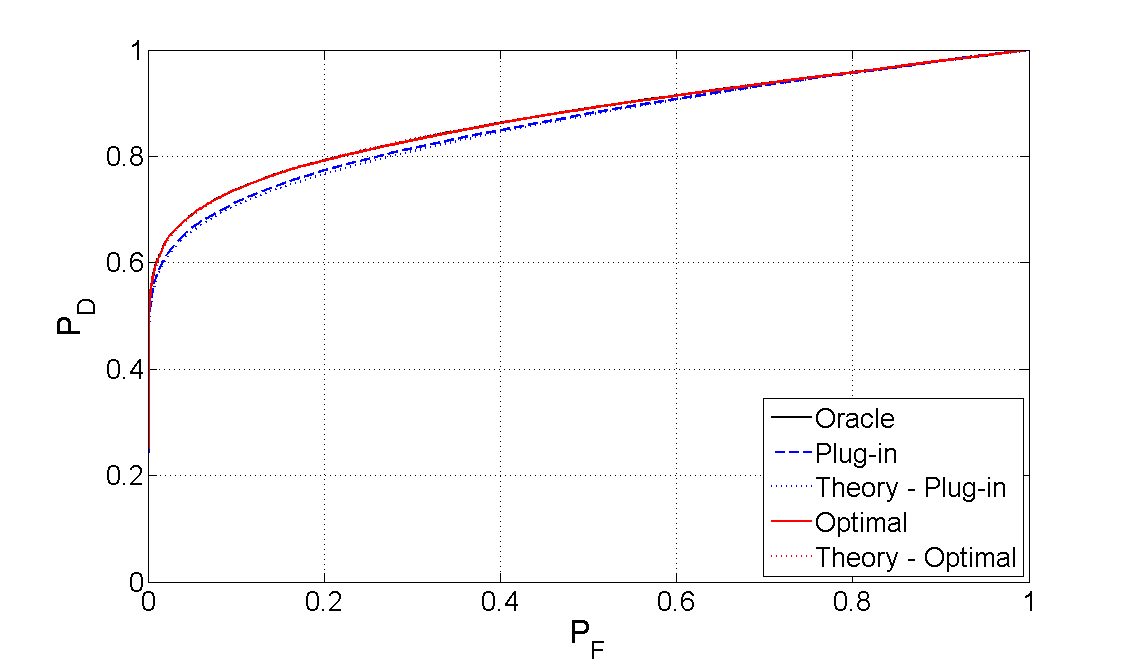
\includegraphics[width=3.5in]{figures/roc_curves.png}
\caption{Empirical and theoretical ROC curves for the oracle, plug-in, and optimal matched subspace detectors. Empirical ROC curves were simulated with $n=100$, $m=50$, $k=2$, $\widehat{k}=2$, $\sigma_1=5$, $\sigma_2=0.5$. However, as $\sigma_2$ is below the critical threshold, $k_{\text{eff}} = 1$. The empirical ROC curves were computed using 2000 test samples and averaged over 25 trials using algorithms 2 and 4 of \cite{fawcett2006introduction}. The theoretical ROC curves were computed as described in Section \ref{sec:roc}. Because $\widehat{k}\neq k_{\text{eff}}$, we observe a performance gain when using the optimal detector. In fact, the optimal detector operates at almost the same $(P_F, P_D)$ as the oracle detector. The theoretical ROC curves match the empirical ones for each detector.}
\label{fig:roc}
\end{figure}

\begin{figure}
\centering
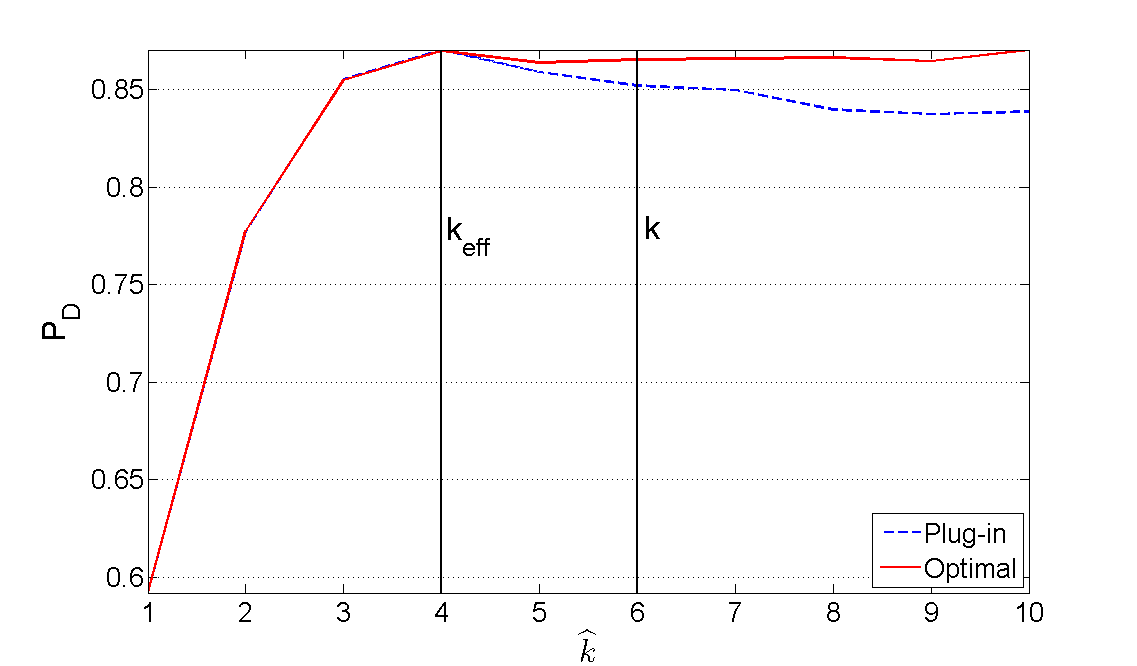
\includegraphics[width=3.5in]{figures/k_hat_graph.png}
\caption{Empirical exploration of the achieved probability of detection, $P_D$, for a fixed probability of false alarm, $P_F=0.01$, for various $\widehat{k}$. For the simulation, $n=100$, $m=50$, $k=6$, $\Sigma^{1/2} = \diag({\bf{5,4,3,2}},0.6,0.5)$ so that $k_{\text{eff}}=4$. $P_D$ calculation was computed using 2000 test samples and averaged over 25 trials. The optimal $\widehat{k}$ resulting in the largest $P_D$ is not the true $k$, but rather $k_\text{eff}$.}
\label{fig:khat}
\end{figure}

\begin{figure}
\centering
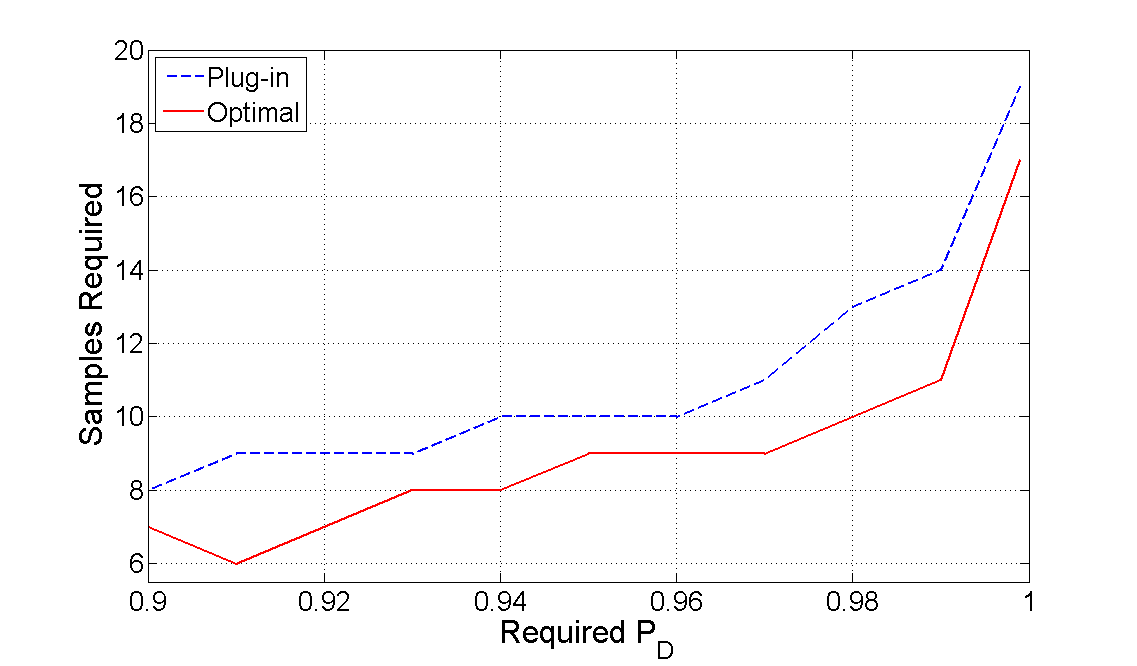
\includegraphics[width=3.5in]{figures/samples_graph.png}
\caption{Empirical exploration of the number of test samples required to achieve a desired $P_F=0.001$ for different $P_D$. In this setup, $N$ test samples are averaged together and then sent to each detector. For the simulation, $n=100$, $m=50$, $k=6$, $\widehat{k}=6$,$\Sigma^{1/2} = \diag({\bf{3,2}},0.5,0.4,0.3,0.2)$ so that $k_{\text{eff}}=2$. $P_D$ calculation was computed using 2000 test samples and averaged over 10 trials. Because the optimal detector only uses $k_\text{eff}$ dimensions, it requires less test samples to achieve a desired $(P_F, P_D)$ than the plug-in detector.}
\label{fig:samples}
\end{figure}

\section{Simulation Results and Discussion}\label{sec:disc}

\subsection{ROC curves}

Evident in Figure \ref{fig:roc}, the theoretical ROC curves match the empirical ROC curves. Our saddlepoint approximation to the CDF of a weighted sum of independent chi square random variables is valid. As evident by their ROC curves, the optimal detector operates at almost the same $(P_F, P_D)$ as the oracle detector. Therefore, the random matrix theory approximations of unknown parameters are very accurate. Finally, we note the sub-optimality of the plug-in detector. This is expected as it incorrectly assumes that estimated eigenvalues and eigenvectors are exact.

\subsection{Optimality of $k_\text{eff}$}

Evident in Figure \ref{fig:khat}, the optimal $\widehat{k}$ id $k_\text{eff}$. Underestimating $k_\text{eff}$ drastically decreases performance for both detectors. However, the plug-in and optimal detectors operates at roughly the same $P_D$ showing that the different shrinkage weights applied by each detector do not make a difference in detection ability. When overestimating $k_\text{eff}$, the plug-in detector observes a decrease in performance while the optimal detector maintains the same performance as if $\widehat{k}=k_\text{eff}$. Thus, we do not pay a price for overestimating our dimension with the optimal detector. This makes sense because the optimal detector will only sum to a maximum of $k_\text{eff}$ indices as evident in (\ref{eq:rmt stat}). As if often the case, the dimension is purposefully overestimated to ensure that all signal dimensions are included. However as evident in Figure \ref{fig:khat}, doing so with the plug-in detector will degrade performance. In fact, even if $\widehat{k}=k$, the plug-in detector still is suboptimal in this example. Only when $\widehat{k}=k_\text{eff}$ will the optimal performance be achieved.

\subsection{Averaging over Test Samples}

As evident in Figure \ref{fig:samples}, the optimal detector requires less samples than the plug-in detector to achieve a desired $(P_F, P_D)$. This arises from the fact that the optimal detector ignores noisy signal components while the plug-in detector uses them. Because each test sample is pruned to ignore noisy components, we can average less samples to achieve a desired accuracy.

\section{Conclusion}\label{sec:concl}
We have derived three stochastic matched subspace detectors. Through an ROC analysis, we have demonstrated the sub-optimality of the plug-in detector. This arises from the false assumption that estimated eigenvalues and eigenvectors of the sample signal covariance matrix are exact estimates of the true eigenvalues and eigenvectors of our signal covariance matrix. By using random matrix theory to characterize the accuracy of eigenvalues and eigenvectors estimates from limited training data, we have derived an optimal detector. ROC analysis demonstrated that the optimal detector outperforms the plug-in detector. This arises from the optimal detector using the effective number of signal subspace dimensions, $k_\text{eff}$, which was shown to be the optimal dimension estimate for a matched subspace detection problem. Reweighing (or shrinking) dimensions was shown to have little effect on detector performance which is controlled by using the effective dimension, $k_\text{eff}$.


% if have a single appendix:
%\appendix[Proof of the Zonklar Equations]
% or
%\appendix  % for no appendix heading
% do not use \section anymore after \appendix, only \section*
% is possibly needed

% use \appendices with more than one appendix
% then use \section to start each appendix
% you must declare a \section before using any
% \subsection or using \label (\appendices by itself
% starts a section numbered zero.)
%


%\appendices
%\section{Proof of the First Zonklar Equation}
%Appendix one text goes here.
%
%% you can choose not to have a title for an appendix
%% if you want by leaving the argument blank
%\section{}
%Appendix two text goes here. 